\documentclass[journal,12pt,twocolumn]{IEEEtran}

\usepackage{enumitem}
\usepackage{amsmath}
\usepackage{amssymb}
\usepackage{gensymb}
\usepackage{graphicx}
\usepackage{txfonts}         
\usepackage{listings}
\usepackage{lstautogobble}
\usepackage{mathtools}
\usepackage{bm}
\usepackage{hyperref}
\usepackage{polynom}
\usepackage{capt-of}
\usepackage{circuitikz}
\newcommand{\solution}{\noindent \textbf{Solution: }}
\providecommand{\pr}[1]{\ensuremath{\Pr\left(#1\right)}}
\providecommand{\brak}[1]{\ensuremath{\left(#1\right)}}
\providecommand{\cbrak}[1]{\ensuremath{\left\{#1\right\}}}
\providecommand{\sbrak}[1]{\ensuremath{\left[#1\right]}}
\providecommand{\mean}[1]{E\left[ #1 \right]}
\providecommand{\var}[1]{\mathrm{Var}\left[ #1 \right]}
\providecommand{\der}[1]{\mathrm{d} #1}
\providecommand{\gauss}[2]{\mathcal{N}\ensuremath{\left(#1,#2\right)}}
\providecommand{\mbf}{\mathbf}
\providecommand{\abs}[1]{\left\vert#1\right\vert}
\providecommand{\norm}[1]{\left\lVert#1\right\rVert}
\providecommand{\z}[1]{{\mathcal{Z}}\{#1\}}
\providecommand{\ztrans}{\overset{\mathcal{Z}}{ \rightleftharpoons}}
\providecommand{\system}[1]{\overset{\mathcal{#1}}{ \longleftrightarrow}}
\providecommand{\laplaceinv}[1]{{\mathcal{L}^{-1}\ensuremath{\left[#1\right]}}}
\providecommand{\parder}[2]{\frac{\partial}{\partial #2} \brak{#1}}

\let\StandardTheFigure\thefigure
\let\vec\mathbf

\numberwithin{equation}{section}
\renewcommand{\thefigure}{\theenumi}
\renewcommand\thesection{\arabic{section}}

\newcommand{\myvec}[1]{\ensuremath{\begin{pmatrix}#1\end{pmatrix}}}
\newcommand{\mydet}[1]{\ensuremath{\begin{vmatrix}#1\end{vmatrix}}}
\newcommand{\define}{\stackrel{\triangle}{=}}

\DeclareMathOperator*{\argmin}{arg\,min}
\DeclareMathOperator*{\argmax}{arg\,max}


\lstset {
	frame=single, 
	breaklines=true,
	columns=fullflexible,
	autogobble=true
}             
   


\begin{document}
                             
\title{ Digital Signal Processing  \\ 
	\Large EE3900
	%: Linear Systems and Signal Processing \\ \large Indian Institute of Technology Hyderabad \\ \vspace*{12pt} \textbf{Circuits and Transforms}
}
\author{I Sai Pradeep \\ \normalsize AI21BTECH11013 \\ \vspace*{20pt} \normalsize \today  }
 \maketitle 
 \tableofcontents
 \section{Definitions}
\begin{enumerate}[label=\arabic*.,ref=\thesection.\theenumi]
\numberwithin{equation}{section}
\numberwithin{figure}{section}
\item The unit step function is 
\begin{align}
\label{eq:unit-step}
u(t) =
\begin{cases}
1 & t > 0
\\
	\frac{1}{2} & t = 0
\\
0 & t < 0
\end{cases}
\end{align}
\item The Laplace transform of $g(t)$ is defined as 
\begin{align}
	G(s) = \int_{-\infty}^{\infty} g(t) e^{-st}\, dt
\end{align}
 \end{enumerate}

 \section{Laplace Transform}
\begin{enumerate}[label=\arabic*.,ref=\thesection.\theenumi]
\numberwithin{equation}{section}
\item In the circuit, the switch S is connected to position P for a long time so that the charge on the capacitor
	becomes $q_1 \, \mu C$. Then S is switched to position Q.  After a long time, the charge on the capacitor is
		$q_2 \, \mu C$.
		\begin{figure}[!ht]
			\centering
			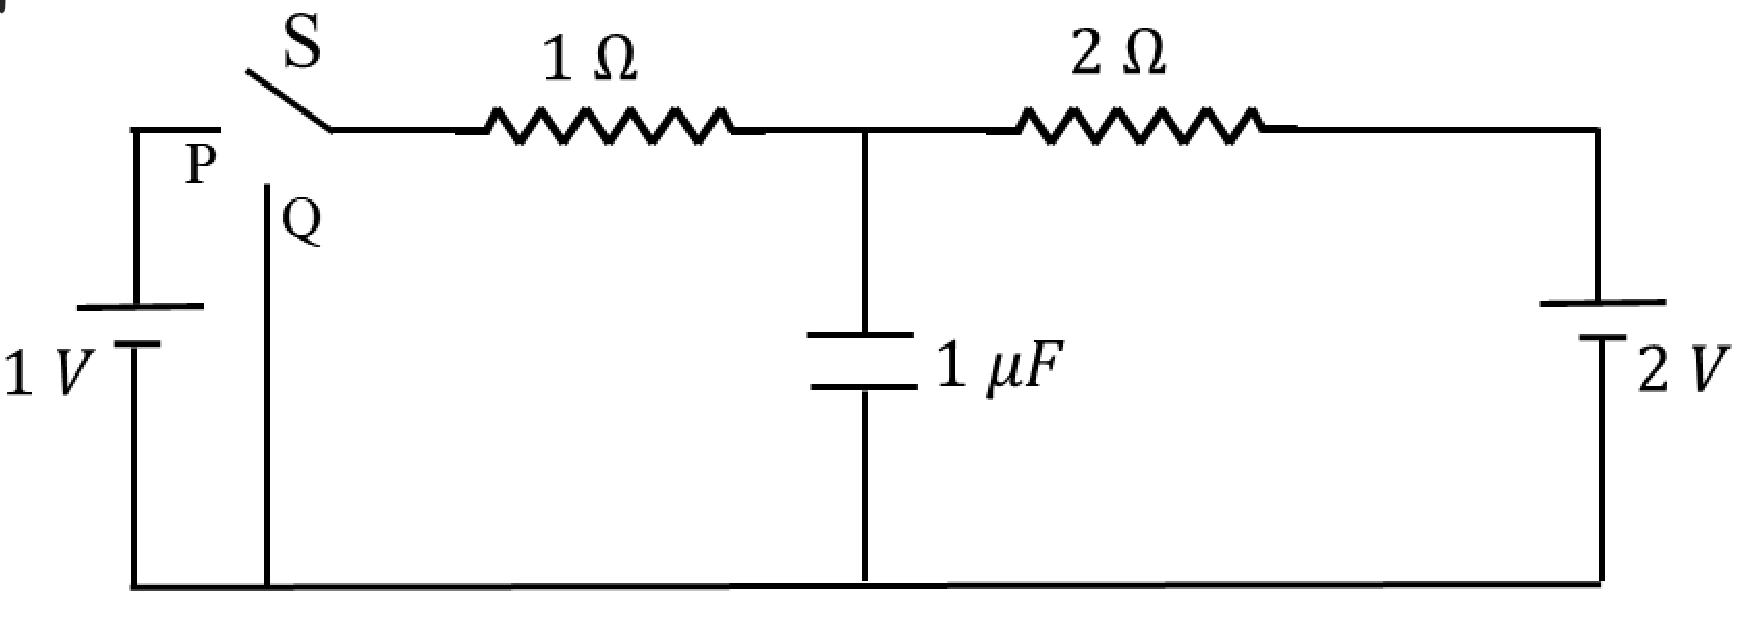
\includegraphics[width=\columnwidth]{figs/ckt.jpg}
			\caption{}
			\label{fig:ckt}
\end{figure}
\item Draw the circuit using latex-tikz.\\
\solution The following code yields Fig.\ref{fig:qn}
\begin{lstlisting}
wget https://github.com/Pradeep8802/EE3900-Digital-Signal-Processing/blob/main/cktsig/Tikz%20Circuits/2.2.tex
\end{lstlisting}
\begin{figure}[!ht]
 \centering
  \begin{circuitikz}[scale=0.7] 
\draw (0,0) to [battery1,l_=$1V$] ++(0,-3)
	
	to ++(11.5,0) to [battery1,l_=$2V$,invert]++(0,3)
	
	to [american resistor,l_=$2\Omega$] ++(-6,0)
	
	to [capacitor,l_=$1 \mu F$] ++(0,-3);
	
	\draw (0,0) to ++(0.7,0) node[anchor=north east]{P};
	
	\draw (1,-3) to ++(0,2.6)node[anchor=north west]{Q};
	
	\draw (4.5,0) to ++(1.5,0);
	
	\draw (4.5,0) to [american resistor,l_=$1\Omega$]++(-3,0) 
	
	to ++(-0.8,0.4)node[anchor=south west]{S};
;
\end{circuitikz}

\caption{Given Circuit}
\label{fig:qn}
\end{figure}

\item Find $q_1$.\\
\solution
Before switching S to Q:
\begin{figure}
 %\centering
   \begin{circuitikz}[scale=0.7]
	\draw (0,0) to [battery1,l_=$1V$] ++(0,-3)
	to ++(11.5,0) to [battery1,l_=$2V$,invert]++(0,3)
	to [american resistor,l_=$2\Omega$] ++(-6,0)
	to [capacitor,l_=$1 \mu F$] ++(0,-3);
	\draw (0,0) to ++(2.5,0);
	\draw (4.5,0) to ++(1.5,0);
	\draw (4.5,0) to [american resistor,l_=$1\Omega$]++(-2,0) ;
\end{circuitikz}

\caption{Before switching S to Q}
%\label{fig:c1}
\end{figure}
At steady state, which achieved when switch S is at P for long time capacoitor behaves as an open switch, hence current through capacitor is $0$,
Let $i$ be the current flowing in the circuit at steady state. Applying KVL ,
\begin{align}
1-i-2i-2=0\\
3i=-1 \Rightarrow i=\frac{-1}{3}A
\end{align}
Potential Difference across the capacitor at steady state is
\begin{align}
1-\brak{\frac{-1}{3}}=\frac{4}{3}V\\
q_1=\frac{4}{3} \cdot 1\\
=\frac{4}{3} \mu C
\end{align}
	\item Show that the Laplace transform of $u(t)$ is $\frac{1}{s}$ and find the ROC.\\
	\solution We know that Laplace Transform fo function $f(t)$ is given as $F(s)$,
	\begin{align}
		\label{eq:LaplaceTrans}
	F(s)&= \int_{0}^{\infty} f(t)e^{-st} \,dt \\
\end{align}
For $u(t)$, we have,
\begin{align}
	F(s)&=\int_{0}^{\infty} u(t)e^{-st} \,dt
\end{align}
	Using \eqref{eq:unit-step},
	\begin{align}
	F(s)&=\int_{0}^{\infty} u(t)e^{-st} \,dt\\
	&=\int_{0}^{\infty} e^{-st} \,dt\\
	&=-\brak{0-\frac{1}{s}}\\
	&=\frac{1}{s}
	\end{align}
	ROC is $ Re(s)>0$ since for $s>0$, $e^{-st}<\infty$ for $t \to \infty$
	\begin{figure}[!ht]
			\centering
			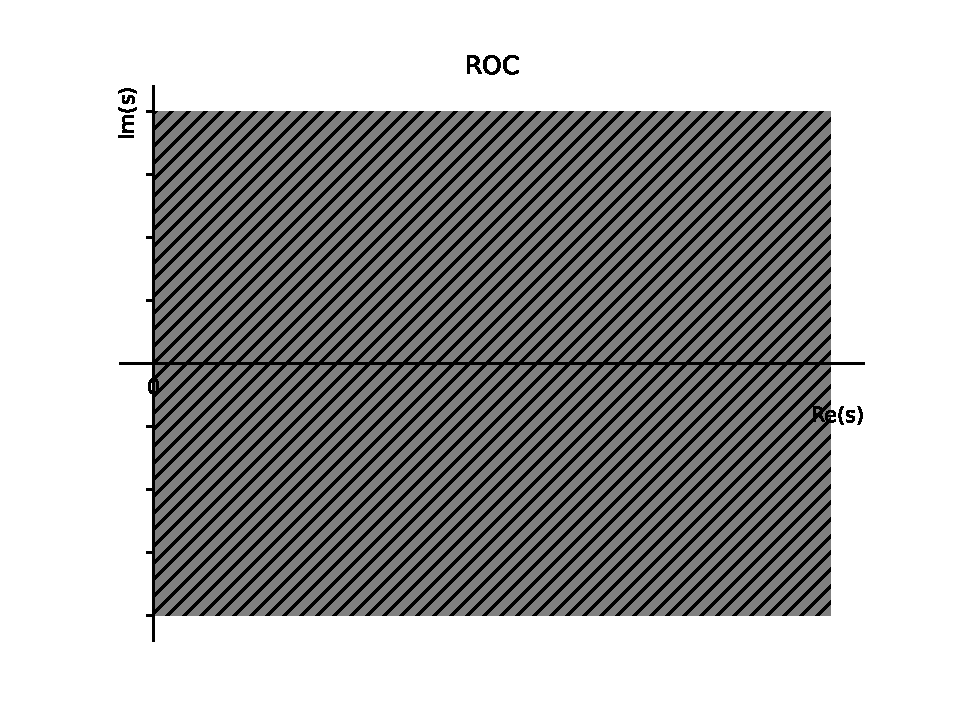
\includegraphics[width=\columnwidth]{figs/2.4}
			\caption{}
			\label{fig:roc1}
\end{figure}
	\item Show that 
		\begin{align}
			e^{-at}u(t) \system{L} \frac{1}{s+a}, \quad a > 0
		\end{align}
		and find the ROC.\\
		\solution From \ref{eq:LaplaceTrans},
		\begin{align}
		F(s)&=\int_{0}^{\infty} u(t)e^{-at}e^{-st} \,dt\\
		&=\int_{0}^{\infty} u(t)e^{-\brak{s+a}t} \,dt\\
		&=\int_{0}^{\infty} e^{-\brak{s+a}t} \,dt\\
		&=-\brak{0-\frac{1}{s+a}}\\
		&=\frac{1}{s+a}
		\end{align}
		ROC is
		\begin{align}
		Re(s)+a>0 \Rightarrow  Re(s)>-a
		\end{align}
		\begin{figure}[!ht]
			\centering
			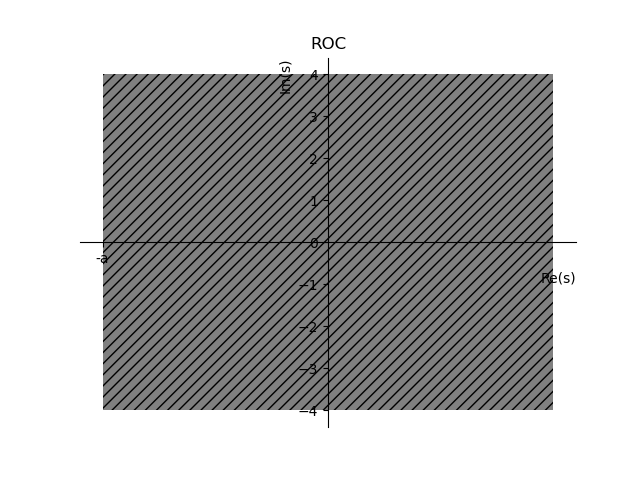
\includegraphics[width=\columnwidth]{figs/2.5}
			\caption{}
			\label{fig:roc2}
\end{figure}
	\item Now consider the following resistive circuit transformed from 
			Fig. \ref{fig:ckt}
		\begin{figure}[!ht]
			\centering
			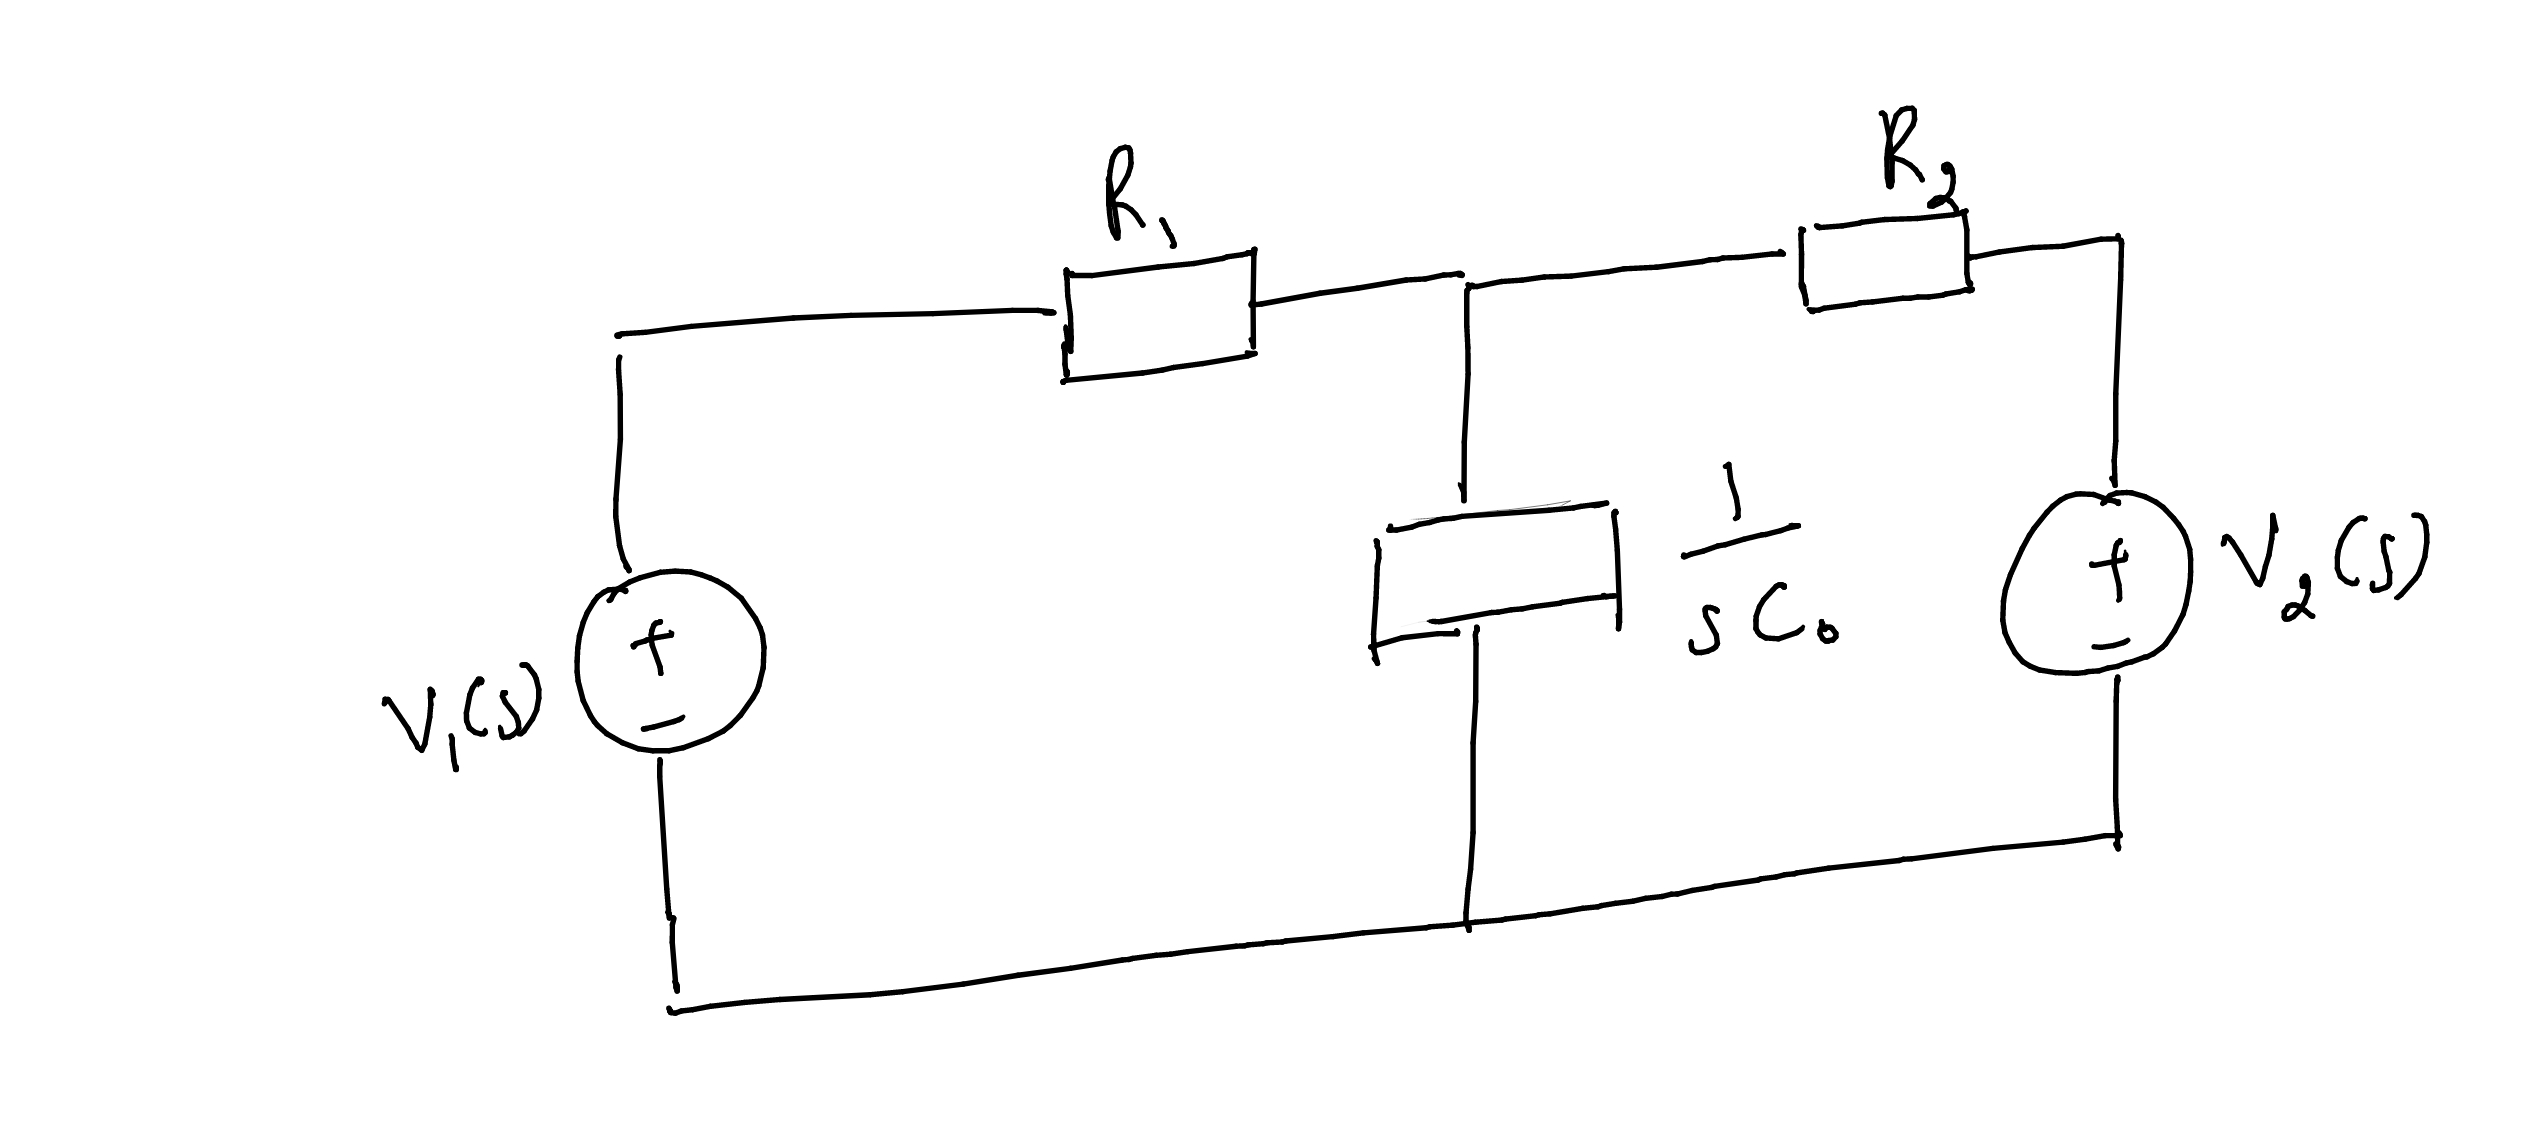
\includegraphics[width=\columnwidth]{figs/lap-ckt.jpg}
			\caption{}
			\label{fig:lap-ckt}
\end{figure}
		where 
		\begin{align}
			u(t) \system{L} V_1(s)
			\\
			2u(t) \system{L} V_2(s)
		\end{align}
		Find the voltage across the capacitor $V_{C_0}(s)$.\\
		\solution
		\begin{align}
		R_{eff}=\frac{\frac{2}{2}+\frac{1}{1}}{1+\frac{1}{2}}
		=\frac{4}{3} \Omega\\
		V_{eff}=\frac{1}{1+\frac{1}{2}}
		=\frac{2}{3}V
		\end{align}
		%Effective Circuit in Laplacian Space is
\begin{align}
V_{C_0}(s)&=V_{S}(s)\frac{C_{0}}{C_{0}+R_{eff}}\\
&=\brak{\frac{4}{3s}}\brak{\frac{\frac{1}{s}}{\frac{1}{s}+\frac{4}{3}}}\\
\label{eq:laptr}
&=\frac{4}{s\brak{4s+3}}
\end{align}
	\item Find $v_{C_0}(t)$.  Plot using python.\\
	\solution Using \eqref{eq:laptr},
	\begin{align}
	\frac{4}{s\brak{4s+3}}&=\frac{4}{3s}-\frac{4}{3(\frac{3}{2}+s)}
	\end{align}
	Apply inverse Laplacian Transform,
	\begin{align}
	V_{C_0}(s)\system{L^{-1}}V_{C_0}(t)\\
	\laplaceinv{V_{C_0}(s)}&=\laplaceinv{\frac{4}{3s}-\frac{4}{3(\frac{3}{2}+s)}}\\
&=	\laplaceinv{\frac{4}{3s}}-\frac{4}{3}\laplaceinv{\frac{1}{\frac{3}{2}+s}}
\end{align}
Since,
\begin{align}
\laplaceinv{\frac1s}&=u(t)\\
\laplaceinv{\frac{1}{s-a}}&=e^{at}u(t)
\end{align}
Using the above equations,
\begin{align}
V_{C_0}(t)=\frac{4}{3}\brak{ 1-e^{\frac{-3}{2} t}}u(t)
	\end{align}
	\begin{figure}[!ht]
			\centering
			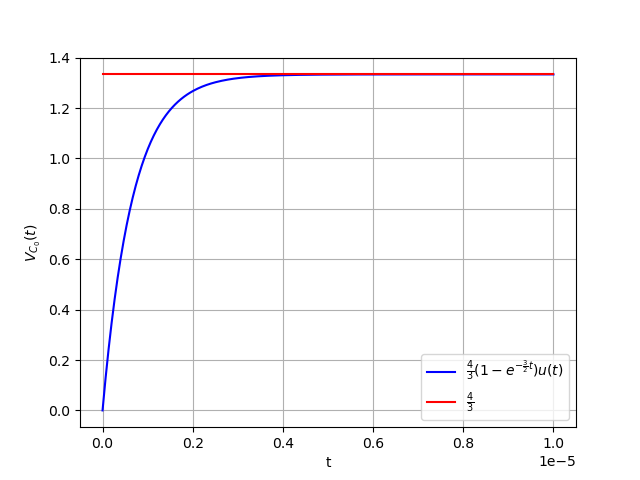
\includegraphics[width=\columnwidth]{figs/2.7.png}
			\caption{Plot of $V_{C_0}(t)$}
			%\label{fig:lap-ckt}
\end{figure}
	\item Verify your result using ngspice.\\
\solution \begin{figure}[!ht]
			\centering
			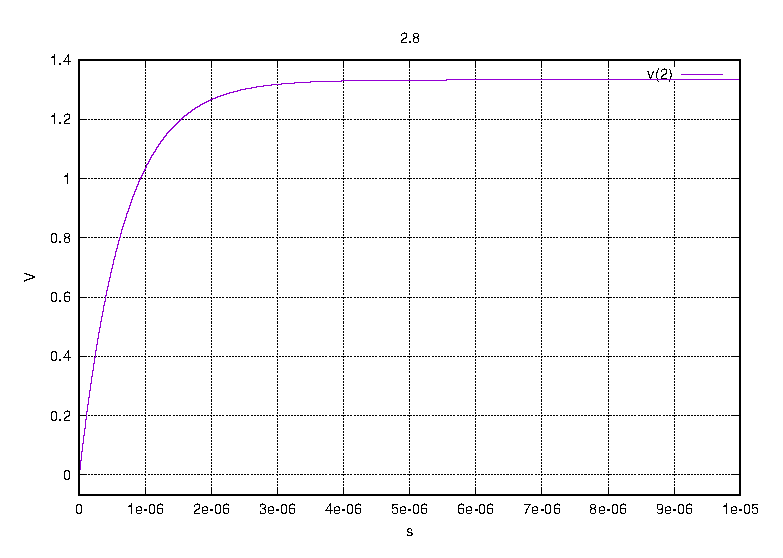
\includegraphics[width=\columnwidth]{figs/2.8}
			\caption{}
			\label{fig:ngspice}
\end{figure}
\end{enumerate}

 \section{Initial Conditions}
\begin{enumerate}[label=\arabic*.,ref=\thesection.\theenumi]
\numberwithin{equation}{section}
\item Find $q_2$ in Fig. \ref{fig:ckt}.\\
			\solution At steady state capacitor behaves as an open switch. Hence $V_{C_0}=V_{1 \Omega}$.\\
			Let $i$ be the current in the circuit. Using KVL,
			\begin{align}
				2-2i-i=0 \implies i=\frac{2}{3}\\
				V_{1 \Omega}=i \times 1= \frac{2}{3} V\\
			V_{C_0}=\frac{q_2}{C_0}=V_{1 \Omega}=\frac{2}{3}\\
			\implies q_2=\frac{2}{3} \mu C
			\end{align}
\item Draw the equivalent $s$-domain resistive circuit when S is switched to position Q.  Use variables $R_1, R_2, C_0$ for the passive elements.
Use latex-tikz.
		\label{prob:init}
		\\\solution 
	\begin{figure}[!ht]
 \centering
 \begin{circuitikz}[scale=1.5]
  \draw (0,0) to [generic,l=$R_1$]++(2,0) to[generic,l=$R_2$]++(2,0)
  to [battery1,l=$\frac2s V$]++(0,-2) to ++(-2,0)
  to [generic,l=$\frac{1}{sC_0}$]++(0,1) to [battery1,l=$\frac{4}{3s}V$,invert]++(0,1);
  \draw (0,0) to ++(0,-2) to ++(2,0);
  \end{circuitikz}

\caption{After switching S to Q}
\label{fig:sq}
\end{figure}
		\item $V_{C_0}(s)$ = ? \\
		\solution Let voltage across capacitor be $V$. Using KCL at node in Fig. \ref{fig:sq}
\begin{align}
    \frac{V - 0}{R_1} + \frac{V - \frac{2}{s}}{R_2} + sC_0\brak{V - \frac{4}{3s}} = 0 \\
\implies V_{C_0}(s) = \frac{\frac{2}{sR_2} + \frac{4C_0}{3}}{\frac{1}{R_1} + \frac{2}{R_2} + sC_0}
\label{eq:v2-s}
\end{align} 
	\item $v_{C_0}(t)$ = ? Plot using python.\\
	\solution From \eqref{eq:v2-s},
\begin{align}
    &V_{C_0}(s) = \frac{4}{3}\brak{\frac{1}{\frac{1}{C_0}\brak{\frac{1}{R_1} + \frac{1}{R_2}}+s}} \nonumber \\
    &+ \frac{2}{R_2\brak{\frac{1}{R_1} +\frac{1}{R_2}}}\brak{\frac{1}{s} - \frac{1}{\frac{1}{C_0}\brak{\frac{1}{R_1} + \frac{1}{R_2}} + s}}
\end{align}
Taking an inverse Laplace Transform,
\begin{align}
    &v_{C_0}(t) = \frac{4}{3}e^{-\brak{\frac{1}{R_1} + \frac{1}{R_2}}\frac{t}{C_0}}u(t) \nonumber \\ 
    &+ \frac{2}{R_2\brak{\frac{1}{R_1}+\frac{1}{R_2}}}\brak{1 - e^{-\brak{\frac{1}{R_1} + \frac{1}{R_2}}\frac{t}{C_0}}}u(t)
\end{align}
Substituting values gives
\begin{align}
    v_{C_0}(t) = \frac{2}{3}\brak{1 +e^{-\brak{1.5 \times 10^6}t}}u(t)
    \label{eq:v2-t}
\end{align}
\begin{figure}[!ht]
			\centering
			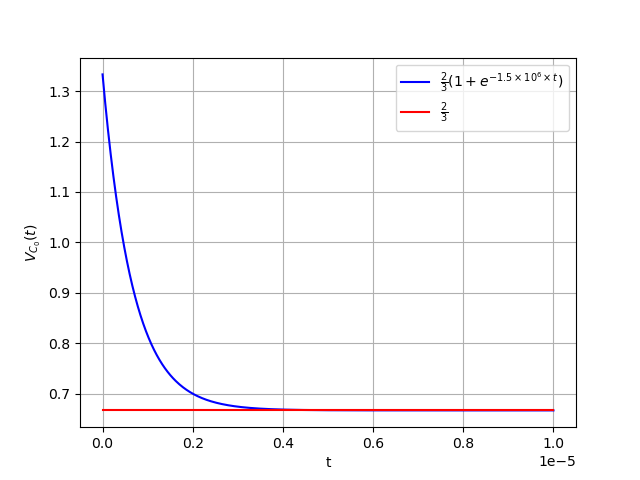
\includegraphics[width=\columnwidth]{figs/3.4.png}
			\caption{Plot of $V_{C_0}(t)$}
			%\label{fig:lap-ckt}
\end{figure}
	\begin{figure}[!ht]
	\centering
	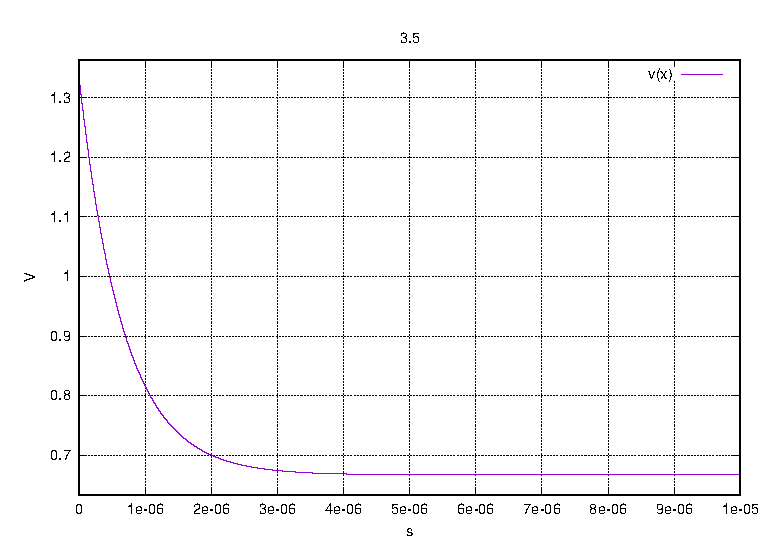
\includegraphics[width=\columnwidth]{figs/3.5}
	\caption{ngspice plot of $V_{C_0}(t)$} 
	\label{fig:ngspice2}
\end{figure}
	\item Verify your result using ngspice.\\
	\solution The figure \ref{fig:ngspice2} verifies our result. 

	\item Find $v_{C_0}(0-), v_{C_0}(0+)$ and  $v_{C_0}(\infty) $.\\
\solution From the initial conditions,
\begin{align}
    v_{C_0}(0-) = \frac{q_1}{C} = {\frac{4}{3}}{V}
\end{align}
Using \eqref{eq:v2-t},
\begin{align}
    v_{C_0}(0+) &= \lim_{t \to 0+}v_{C_0}(t) = {\frac{4}{3}}{V} \\
    v_{C_0}(\infty) &= \lim_{t \to \infty}v_{C_0}(t) = {\frac{2}{3}}{V}
\end{align}


	\end{enumerate}

\end{document}
